
%package list
\documentclass{article}
\usepackage{amsmath}
\usepackage[top=3cm, bottom=3cm, outer=3cm, inner=3cm]{geometry}
\usepackage{multicol}
\usepackage{graphicx}
\usepackage{url}
%\usepackage{cite}
\usepackage{hyperref}
\usepackage{array}
%\usepackage{multicol}
\newcolumntype{x}[1]{>{\centering\arraybackslash\hspace{0pt}}p{#1}}
\usepackage{natbib}
\usepackage{pdfpages}
\usepackage{multirow}
\usepackage[normalem]{ulem}
\useunder{\uline}{\ul}{}
\usepackage{svg}
\usepackage{xcolor}
\usepackage{listings}
\lstdefinestyle{ascii-tree}{
    literate={├}{|}1 {─}{--}1 {└}{+}1 
  }
\lstset{basicstyle=\ttfamily,
  showstringspaces=false,
  commentstyle=\color{red},
  keywordstyle=\color{blue}
}
%\usepackage{booktabs}
\usepackage{caption}
\usepackage{subcaption}
\usepackage{float}
\usepackage{array}

\newcolumntype{M}[1]{>{\centering\arraybackslash}m{#1}}
\newcolumntype{N}{@{}m{0pt}@{}}


%%%%%%%%%%%%%%%%%%%%%%%%%%%%%%%%%%%%%%%%%%%%%%%%%%%%%%%%%%%%%%%%%%%%%%%%%%%%
%%%%%%%%%%%%%%%%%%%%%%%%%%%%%%%%%%%%%%%%%%%%%%%%%%%%%%%%%%%%%%%%%%%%%%%%%%%%
\newcommand{\itemEmail}{ccapatinta@unsa.edu.pe}
\newcommand{\itemStudent}{Capatinta Almanza Camilo B. A.}
\newcommand{\itemCourse}{Lab. Análisis y Diseño de Algoritmos}
\newcommand{\itemCourseCode}{1702231}
\newcommand{\itemSemester}{IV}
\newcommand{\itemUniversity}{Universidad Nacional de San Agustín de Arequipa}
\newcommand{\itemFaculty}{Facultad de Ingeniería de Producción y Servicios}
\newcommand{\itemDepartment}{Departamento Académico de Ingeniería de Sistemas e Informática}
\newcommand{\itemSchool}{Escuela Profesional de Ingeniería de Sistemas}
\newcommand{\itemAcademic}{2026 - B}
\newcommand{\itemInput}{17/09/2026}
\newcommand{\itemOutput}{21/09/2026}
\newcommand{\itemPracticeNumber}{03}
\newcommand{\itemTheme}{Divide y vencerás Ordenamiento: MergeSort y Quicksort.}
%%%%%%%%%%%%%%%%%%%%%%%%%%%%%%%%%%%%%%%%%%%%%%%%%%%%%%%%%%%%%%%%%%%%%%%%%%%%
%%%%%%%%%%%%%%%%%%%%%%%%%%%%%%%%%%%%%%%%%%%%%%%%%%%%%%%%%%%%%%%%%%%%%%%%%%%%

\usepackage[english,spanish]{babel}
\usepackage[utf8]{inputenc}
\AtBeginDocument{\selectlanguage{spanish}}
\renewcommand{\figurename}{Figura}
\renewcommand{\refname}{Referencias}
\renewcommand{\tablename}{Tabla} %esto no funciona cuando se usa babel
\AtBeginDocument{%
	\renewcommand\tablename{Tabla}
}

\usepackage{fancyhdr}
\pagestyle{fancy}
\fancyhf{}
\setlength{\headheight}{40.51407pt}
\renewcommand{\headrulewidth}{1pt}
\renewcommand{\footrulewidth}{1pt}
\fancyhead[L]{\raisebox{-0.2\height}{
\includegraphics[width=3cm]{img/logo_episunsa.png}}}
\fancyhead[C]{\fontsize{7}{7}\selectfont	\itemUniversity \\ \itemFaculty \\ \itemDepartment \\ \itemSchool \\ \textbf{\itemCourse}}
\fancyhead[R]{\raisebox{-0.2\height}{
\includegraphics[width=1.2cm]{img/logo_abet}}}
\fancyfoot[L]{Estudiante Capatinta C.}
\fancyfoot[C]{\itemCourse}
\fancyfoot[R]{Página \thepage}

% para el codigo fuente
\usepackage{listings}
\usepackage{color, colortbl}
\definecolor{dkgreen}{rgb}{0,0.6,0}
\definecolor{gray}{rgb}{0.5,0.5,0.5}
\definecolor{mauve}{rgb}{0.58,0,0.82}
\definecolor{codebackground}{rgb}{0.95, 0.95, 0.92}
\definecolor{tablebackground}{rgb}{0.8, 0, 0}

\lstset{frame=tb,
	language=bash,
	aboveskip=3mm,
	belowskip=3mm,
	showstringspaces=false,
	columns=flexible,
	basicstyle={\small\ttfamily},
	numbers=none,
	numberstyle=\tiny\color{gray},
	keywordstyle=\color{blue},
	commentstyle=\color{dkgreen},
	stringstyle=\color{mauve},
	breaklines=true,
	breakatwhitespace=true,
	tabsize=3,
	backgroundcolor= \color{codebackground},
}

\begin{document}
	
	\vspace*{10px}
	
	\begin{center}	
		\fontsize{17}{17} \textbf{ Informe de laboratorio \itemPracticeNumber}
	\end{center}
	\centerline{\textbf{\Large Tema: \itemTheme}}
	%\vspace*{0.5cm}	

	\begin{flushright}
		\begin{tabular}{|M{2.5cm}|N|}
			\hline 
			\rowcolor{tablebackground}
			\color{white} \textbf{Nota}  \\
			\hline 
			     \\[30pt]
			\hline 			
		\end{tabular}
	\end{flushright}	

	\begin{table}[h!]
		\begin{tabular}{|x{4.7cm}|x{4.8cm}|x{4.8cm}|}        
			\hline 
			\rowcolor{tablebackground}
			\color{white} \textbf{Estudiante} & \color{white}\textbf{Escuela}  & \color{white}\textbf{Asignatura}   \\
			\hline 
			{\itemStudent \par \itemEmail} & \itemSchool & {\itemCourse \par Semestre: \itemSemester \par Código: \itemCourseCode}     \\
			\hline 			
		\end{tabular}
	\end{table}		
	
	\begin{table}[H]
		\begin{tabular}{|x{4.7cm}|x{4.8cm}|x{4.8cm}|}
			\hline 
			\rowcolor{tablebackground}
			\color{white}\textbf{Laboratorio} & \color{white}\textbf{Tema}  & \color{white}\textbf{Duración}   \\
			\hline 
			\itemPracticeNumber & \itemTheme & 02 horas   \\
			\hline 
		\end{tabular}
	\end{table}
	
	\begin{table}[H]
		\begin{tabular}{|x{4.7cm}|x{4.8cm}|x{4.8cm}|}
			\hline 
			\rowcolor{tablebackground}
			\color{white}\textbf{Semestre académico} & \color{white}\textbf{Fecha de inicio}  & \color{white}\textbf{Fecha de entrega}   \\
			\hline 
			\itemAcademic & \itemInput &  \itemOutput  \\
			\hline 
		\end{tabular}
	\end{table}
	
	\section{Ejercicios/Problemas propuestos }
	
	\subsection{Ejercicio 1}

        Implementa Mergesort para ordenar una lista de registros de estudiantes (código: string, nombre: string, promedio ponderado: float) por promedio ponderado, ingresados por el usuario.

    \lstinputlisting[language=c++, caption={Ejercicio 01: MergeSort ordena lista de registros por promedio ponderado},numbers=left,]{e-n/e1.cpp}

    \begin{itemize}
        \item Primero se solicita la cantidad de estudiantes y se
  ingresan sus datos, los cuales se almacenan en un vector. Luego, MergeSort divide el vector en dos partes pequeñas de forma repetitiva
  hasta que cada parte contiene solo un estudiante. Después compara los promedios de los estudiantes de cada parte y los une nuevamente
  en orden, colocando primero al que tenga el promedio más bajo. Al finalizar, el programa muestra todos los estudiantes ordenados por
  promedio. Este algoritmo es eficiente porque puede ordenar muchos datos con una complejidad de O(n log n).
    \end{itemize}

    \begin{figure}[H]
    \centering
    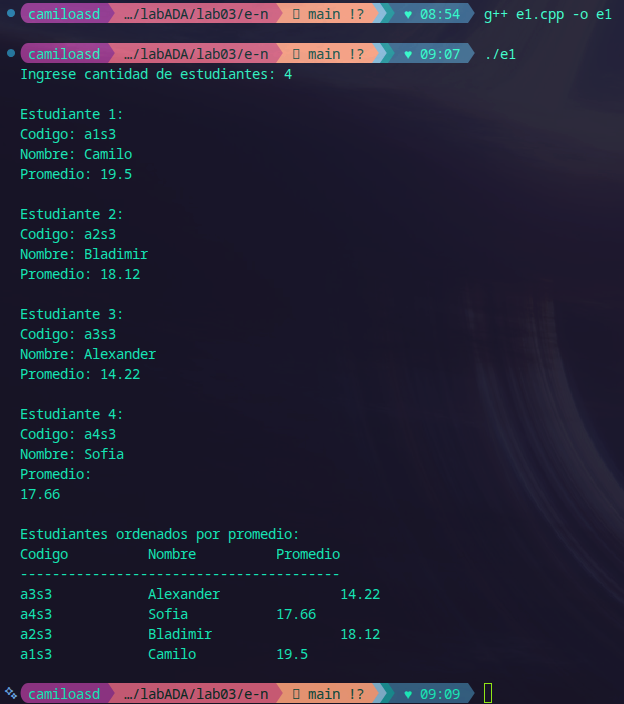
\includegraphics[width=0.8\textwidth]{img/e1.png}
    \caption{Ejecución de e1.cpp}
    \label{fig:diagrama}
    \end{figure}

	\subsection{Ejercicio 2}

        Implementa Quicksort sobre un arreglo de números flotantes. Analiza su rendimiento con pivote fijo y con pivote aleatorio, y explica en qué casos cada estrategia de pivote es más eficiente.
    
    \lstinputlisting[language=c++, caption={Ejercicio 02: Quicksort soobre numeros float },numbers=left,]{e-n/e2.cpp}

    \begin{itemize}
        \item La primera forma utiliza un pivote fijo, que siempre es el último elemento del arreglo, mientras que la segunda
  selecciona un pivote aleatorio. QuickSort funciona eligiendo un pivote y separando los valores menores o iguales a un lado y los
  mayores al otro; luego repite el proceso en cada parte hasta ordenar todo el arreglo. El programa mide el tiempo que tarda cada
  versión y muestra los resultados en milisegundos. El uso de un pivote aleatorio ayuda a evitar divisiones desbalanceadas y reduce la
  posibilidad de que QuickSort alcance su peor caso, cuya complejidad es O(n²); normalmente, ambas versiones tienen un rendimiento
  promedio de O(n log n).
    \end{itemize}

    \begin{figure}[H]
    \centering
    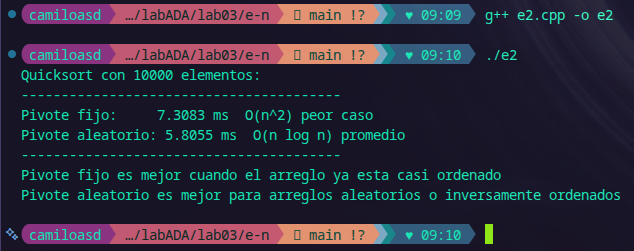
\includegraphics[width=0.9\textwidth]{img/e2.png}
    \caption{Ejecución de e2.cpp}
    \label{fig:diagrama}
    \end{figure}

	\subsection{Ejercicio 3}

		Genera un arreglo de n elementos, ordénalo con Mergesort o Quicksort, implementa una búsqueda binaria para encontrar un elemento dentro del arreglo resultante, y calcula la complejidad temporal total del proceso (ordenamiento + búsqueda) comparándola con la búsqueda secuencial sin ordenamiento previo.
    
		\lstinputlisting[language=c++, caption={Ejercicio 03: Mergesort, Quicksort y busqueda binaria },numbers=left,]{e-n/e3.cpp}

    \begin{itemize}
        \item Primero genera un arreglo de
  tamaño n y guarda una copia sin ordenar. Luego selecciona como objetivo un valor ubicado aproximadamente en la mitad del arreglo. La
  primera estrategia ordena los datos con MergeSort y después busca el número mediante búsqueda binaria. MergeSort tiene complejidad O(n
  log n) y la búsqueda binaria O(log n), pero como es necesario ordenar antes, la complejidad total es O(n log n). La segunda estrategia
  realiza una búsqueda secuencial sobre el arreglo original, revisando los elementos uno por uno hasta encontrar el objetivo, con
  complejidad O(n). El programa mide el tiempo de ambas estrategias y muestra las posiciones encontradas. Para una sola búsqueda, la
  búsqueda secuencial suele ser más conveniente porque no necesita ordenar; sin embargo, si se realizarán muchas búsquedas sobre los
  mismos datos, conviene ordenar una vez con MergeSort y luego usar búsqueda binaria.
    \end{itemize}

    \begin{figure}[H]
    \centering
    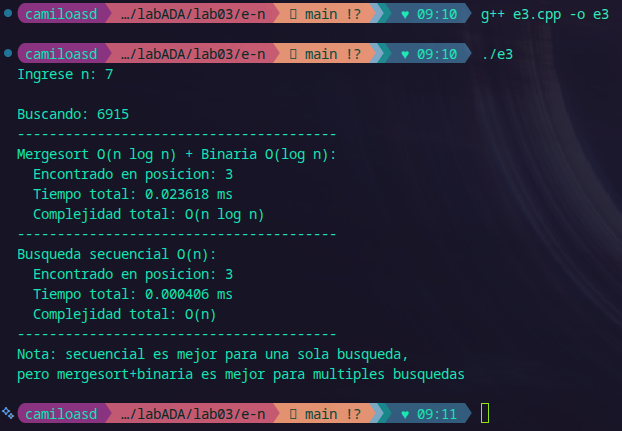
\includegraphics[width=0.8\textwidth]{img/e3.png}
    \caption{Ejecución de e3.cpp}
    \label{fig:diagrama}
    \end{figure}

	\subsection{Ejercicio 4}

		Ordena 10 000 elementos aleatorios y compara los tiempos de ejecución de Mergesort, Quicksort, InsertionSort y Selection Sort.   

		\lstinputlisting[language=c++, caption={Ejercio 04: Tiempos de ejecución de Mergesort, Quicksort, InsertionSort y Selection Sort },numbers=left,]{e-n/e4.cpp}

    \begin{itemize}
        \item Para cada algoritmo se crea una copia del mismo arreglo y se mide cuánto tarda en ordenarlo.
  MergeSort y QuickSort suelen ser más rápidos porque tienen complejidad promedio de O(n log n), mientras que InsertionSort y
  SelectionSort tienen complejidad O(n²), por lo que tardan más con muchos elementos.
    \end{itemize}

    \begin{figure}[H]
    \centering
    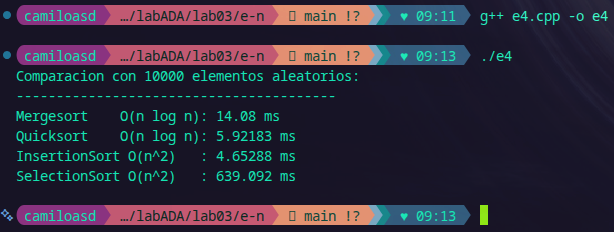
\includegraphics[width=0.8\textwidth]{img/e4.png}
    \caption{Ejecución de e4.cpp}
    \label{fig:diagrama}
    \end{figure}
	
	\subsection{Ejercicio 5}

		Desarrolla una aplicación en C++ que lea un archivo .txt con productos (código, nombre, precio) y los ordene de mayor a menor precio con ambos algoritmos.

		\lstinputlisting[language=c++, caption={Ejercio 05: Aplicación en C++}numbers=left,]{e-n/e5.cpp}

    \begin{itemize}
        \item Lee los datos de productos desde el archivo productos.txt, donde cada producto contiene código, nombre y precio.
  Luego ordena los productos de mayor a menor precio utilizando dos algoritmos: MergeSort y QuickSort. El programa mide el tiempo que
  tarda cada uno, muestra la lista ordenada y permite comparar su rendimiento al trabajar con los mismos datos.
    \end{itemize}

    \begin{figure}[H]
    \centering
    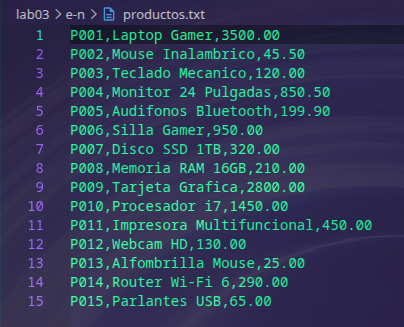
\includegraphics[width=0.95\textwidth]{img/e5(1).png}
    \caption{productos.txt}
    \label{fig:diagrama}
    \end{figure}

   \begin{figure}[H]
    \centering
    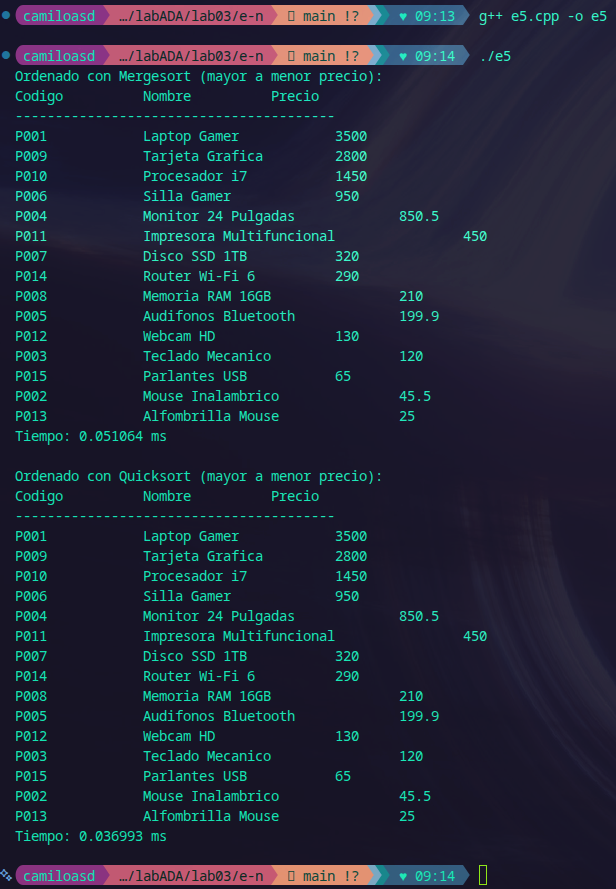
\includegraphics[width=0.95\textwidth]{img/e5(2).png}
    \caption{Ejecución de e5.cpp}
    \label{fig:diagrama}
    \end{figure}


	\section{Cuestionario}

        \begin{enumerate}
            \item La estrategia Divide y vencerás se diferencia de los algoritmos simples porque divide el problema en partes más pequeñas, resuelve cada una por separado y luego combina los resultados. En cambio, algoritmos como InsertionSort o SelectionSort trabajan de forma más directa y suelen requerir más comparaciones o movimientos en casos grandes, por lo que son menos eficientes en volumen de datos.

            \item Mergesort siempre tiene complejidad O(n log n) porque, sin importar el arreglo inicial, se divide repetidamente en dos mitades hasta llegar a subproblemas de tamaño 1 y luego realiza una fusión lineal en cada nivel. Aunque el número de niveles es log n, la cantidad de trabajo por nivel es O(n), por lo que el costo total se mantiene estable en todos los casos.

            \item Quicksort alcanza su peor caso de O(n$^2$) cuando el pivote elegido siempre divide el arreglo de forma muy desbalanceada, por ejemplo cuando el arreglo ya está ordenado o en orden inverso y se toma como pivote el primer o el último elemento. En ese escenario, una parte queda con casi todos los elementos y la otra con pocos, lo que genera muchas llamadas recursivas innecesarias.

            \item En un entorno con restricciones de memoria, Mergesort suele ser menos conveniente si se implementa con copias adicionales durante la fusión, porque necesita memoria auxiliar. QuickSort, al ordenar in-place en muchos casos, resulta preferible cuando el objetivo es ahorrar memoria; sin embargo, si la estabilidad del orden es importante, MergeSort puede ser más apropiado.

            \item Para mejorar el rendimiento práctico de Quicksort se pueden usar pivotes más equilibrados, como el pivote medio o aleatorio, y además aplicar optimizaciones como la ordenación de arreglos pequeños con InsertionSort. Estas estrategias reducen el riesgo de casos desbalanceados y mejoran la velocidad real en entradas grandes.
        \end{enumerate}

	\section{Conclusiones}

	\begin{itemize}
        \item En esta práctica se comprobó que MergeSort y QuickSort son más adecuados para grandes volúmenes de datos que los algoritmos de ordenamiento simple, ya que ambos tienen complejidad promedio de O(n log n). Esto se refleja en la ejecución de los programas, donde la diferencia de tiempo se vuelve evidente al trabajar con arreglos más grandes.

        \item También se evidenció que la elección del pivote y la forma en que se divide el problema afectan directamente el rendimiento de QuickSort. Cuando el particionado es equilibrado, el algoritmo es muy eficiente; cuando no, su comportamiento puede deteriorarse y acercarse a O(n$^2$).

        \item Como conclusión general, el análisis de estos algoritmos permite entender que la eficiencia no depende solo de la complejidad matemática, sino también de la estructura de los datos y del contexto de uso. Por ello, la elección entre MergeSort y QuickSort debe hacerse según la necesidad de estabilidad, memoria disponible y tipo de entrada.
	\end{itemize}

	%\begin{itemize}	
	%	\item Se creo el archivo \textbf{.gitignore} para no considerar los archivos %\textbf{*.class} que son innecesarios hacer seguimiento.
	%\end{itemize}
	%\begin{lstlisting}[language=bash,caption={Creando .gitignore}]
	%	$ vim lab01/.gitignore
	%\end{lstlisting}
	%\begin{lstlisting}[language=bash,caption={lab01/.gitignore}]
	%	*.class
	%\end{lstlisting}
	%\begin{lstlisting}[language=bash,caption={Commit: Creando .gitignore para archivos *.class}]
	%	$ git add .
	%	$ git commit -m "Creando .gitignore para archivos *.class"			
	%	$ git push -u origin main
	%\end{lstlisting}
	
	%\begin{lstlisting}[language=bash,caption={Creando .gitignore}]
	%	$ vim lab01/Insertion.java
	%\end{lstlisting}
	
    
%\clearpage
%\bibliographystyle{apalike}
%\bibliographystyle{IEEEtranN}
%\bibliography{bibliography}
			
\end{document}